\documentclass[tikz,border=4pt]{standalone}
\usepackage{tikz}
\usetikzlibrary{arrows.meta,positioning,calc}
\definecolor{cState}{HTML}{DBEAFE}
\definecolor{cSample}{HTML}{E0F2FE}
\definecolor{cTeacher}{HTML}{FCE7F3}
\definecolor{cResidual}{HTML}{FDE68A}
\definecolor{cOnline}{HTML}{D1FAE5}
\definecolor{cDetail}{HTML}{ECFEFF}
\definecolor{cLoop}{HTML}{059669}

\begin{document}
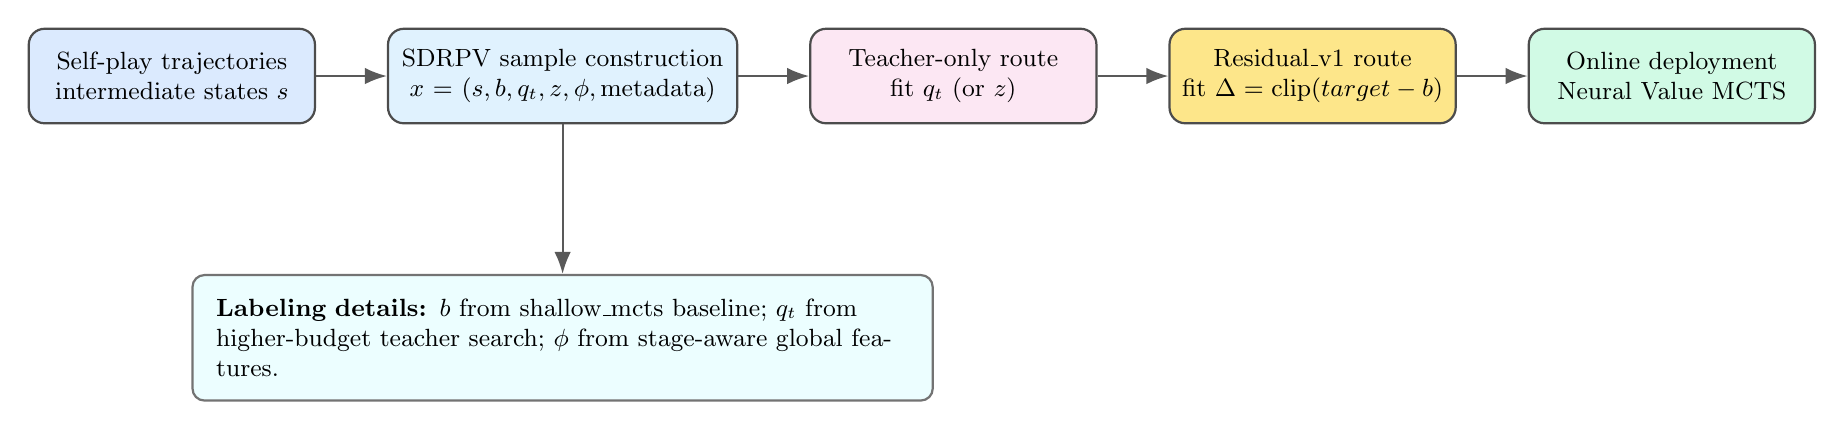
\begin{tikzpicture}[
    font=\small,
    node distance=13mm and 9mm,
    box/.style={draw=black!70, rounded corners=2mm, thick, align=center, minimum height=12mm, text width=34mm},
    arr/.style={-{Latex[length=2.8mm]}, thick, draw=black!65},
    note/.style={draw=black!55, rounded corners=1.5mm, thick, align=left, text width=88mm, fill=cDetail, inner sep=3mm}
]


\node[box, fill=cState, anchor=west] (state) at (0,2.35) {Self-play trajectories\\intermediate states $s$};
\node[box, fill=cSample, right=of state, text width=42mm] (sample) {SDRPV sample construction\\$x=(s,b,q_t,z,\phi,\mathrm{metadata})$};
\node[box, fill=cTeacher, right=of sample] (teacher) {Teacher-only route\\fit $q_t$ (or $z$)};
\node[box, fill=cResidual, right=of teacher] (residual) {Residual\_v1 route\\fit $\Delta=\mathrm{clip}(target-b)$};
\node[box, fill=cOnline, right=of residual] (online) {Online deployment\\Neural Value MCTS};

\node[note, below=19mm of sample] (detail) {
\textbf{Labeling details:}
$b$ from shallow\_mcts baseline; $q_t$ from higher-budget teacher search; $\phi$ from stage-aware global features.
};

\draw[arr] (state) -- (sample);
\draw[arr] (sample) -- (teacher);
\draw[arr] (teacher) -- (residual);
\draw[arr] (residual) -- (online);
\draw[arr] (sample.south) -- (detail.north);

% No online-to-training feedback loop is implemented in code;
% keep the diagram as a one-way pipeline.

\end{tikzpicture}
\end{document}
